
\question{10}
In this problem, there are 4 binary random variables: G = "gray", V = "Vancouver", R="rain", and S="sad". Consider the directed graphical model, shown below, which describes the relationship between these random variables:

\begin{figure}[H]

\begin{minipage}[b]{1.0\linewidth}
  \centerline{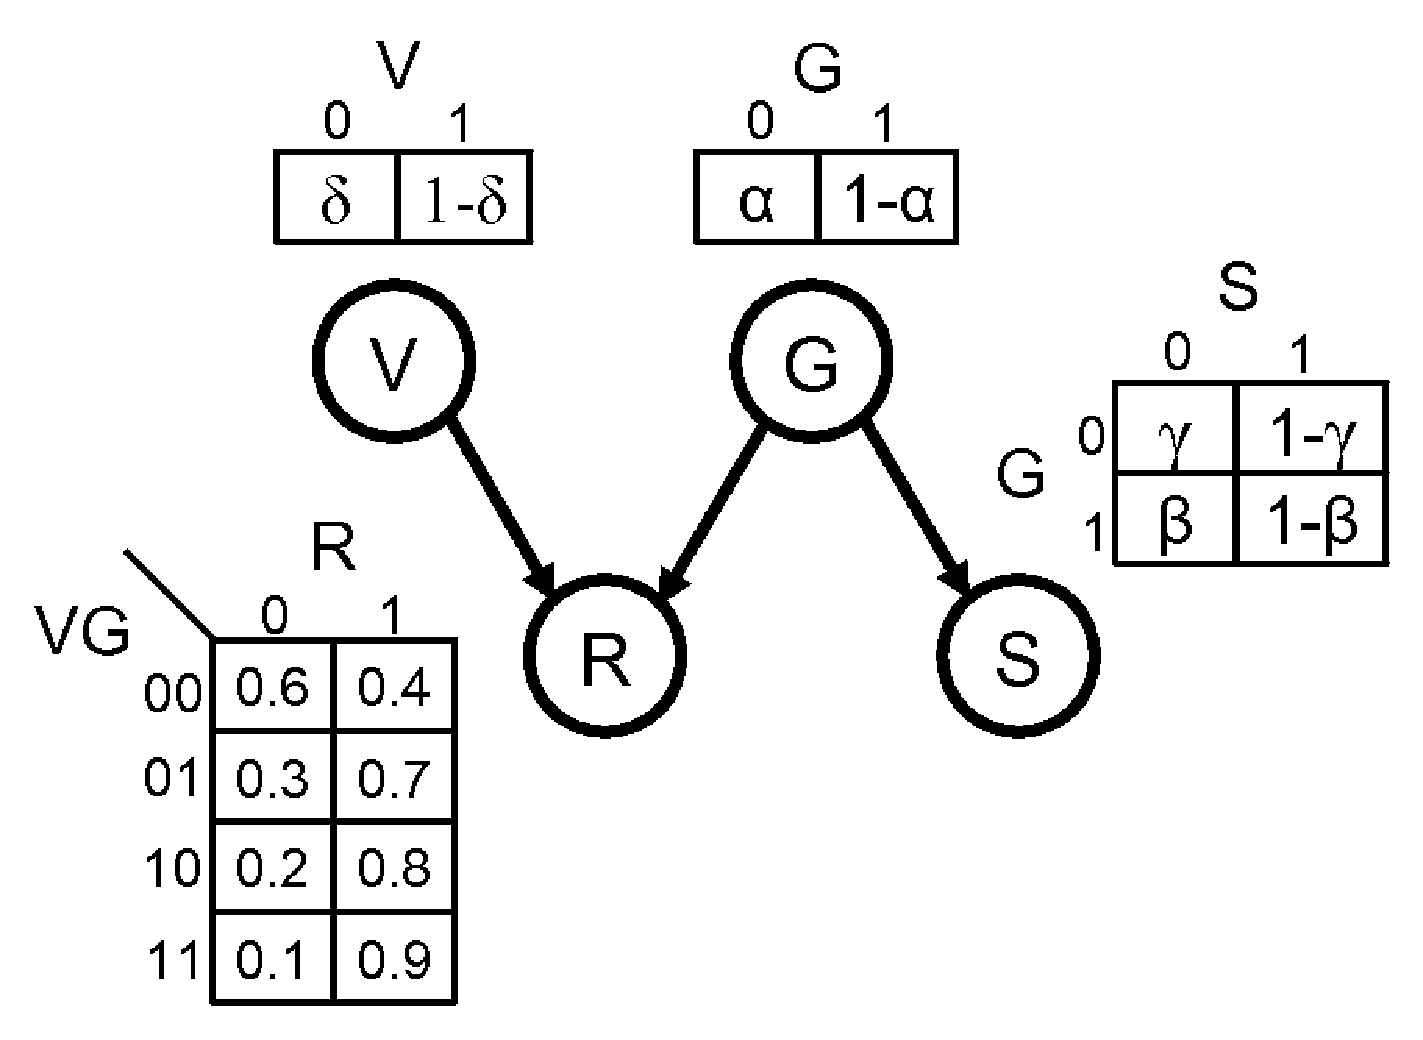
\includegraphics[scale=0.27]{weatherbn.pdf}}
%  \vspace{2.0cm}  
\end{minipage}
\end{figure}


\begin{enumerate}[label=(\alph*)]
\item Write an expression for $P(S=1|V=1)$ in terms of $\alpha, \beta, \gamma, \delta$.
\item Write an expression for $P(S=1|V=0)$. Is this the same or different to $P(S=1|V=1)$? Explain why.
\end{enumerate}
